\begin{figure}[]
  \setlength{\unitlength}{\textwidth}

  \begin{picture}(1,1.2)(0,-0.1)
 
      \put(0.005,0.8){\includegraphics[width=0.5\unitlength]{./chapter-pi_1_pi_2/FnP/gnuplot/freq-1-sig.eps}}
      \put(0.005,0.53){\includegraphics[width=0.5\unitlength]{./chapter-pi_1_pi_2/FnP/gnuplot/freq-05-sig.eps}}
      \put(0.005,0.27){\includegraphics[width=0.5\unitlength]{./chapter-pi_1_pi_2/FnP/gnuplot/freq-04-sig.eps}}
      \put(0.005,-0.01){\includegraphics[width=0.5\unitlength]{./chapter-pi_1_pi_2/FnP/gnuplot/freq-03-sig.eps}}
      
      
      \put(0.505,0.8){\includegraphics[width=0.5\unitlength]{./chapter-pi_1_pi_2/FnP/gnuplot/freq-1.eps}}
      \put(0.505,0.53){\includegraphics[width=0.5\unitlength]{./chapter-pi_1_pi_2/FnP/gnuplot/freq-05.eps}}
      \put(0.505,0.27){\includegraphics[width=0.5\unitlength]{./chapter-pi_1_pi_2/FnP/gnuplot/freq-04.eps}} 
      \put(0.505,-0.01){\includegraphics[width=0.5\unitlength]{./chapter-pi_1_pi_2/FnP/gnuplot/freq-03.eps}}
      
      
      %      \put(0.23,0.00){ $\displaystyle\frac{c}{\rho\mathcal{A}U}$}
      %      \put(0.73,0.00){ $\displaystyle\frac{c}{\rho\mathcal{A}U}$}
      
      \put(0.26,-0.06){$\displaystyle\frac{tU}{D}$}
      \put(0.75,-0.06){$\displaystyle\frac{fD}{U}$}
      
      \put(0.0,0.405){$\displaystyle\frac{V}{U}$}
      \put(0.0,0.66){$\displaystyle\frac{V}{U}$}
      \put(0.0,0.13){$\displaystyle\frac{V}{U}$}
      \put(0.0,0.93){$\displaystyle\frac{V}{U}$}
      
      \put(0.535,0.405){$\displaystyle\mathcal{F}$}
      \put(0.535,0.66){$\displaystyle\mathcal{F}$}
      \put(0.535,0.13){$\displaystyle\mathcal{F}$}
      \put(0.535,0.93){$\displaystyle\mathcal{F}$}
      
      \put(0.434,1.03){\small(a)}
      \put(0.935,1.03){\small(b)}
      \put(0.434,0.760){\small(c)}
      \put(0.935,0.760){\small(d)}
      \put(0.434,0.500){\small(e)}
      \put(0.935,0.5){\small(f)}
      \put(0.434,0.220){\small(g)}
      \put(0.935,0.220){\small(h)}
      
      \put(0.65,0.82){\small$f_g$}
      \put(0.92,0.82){\small$f_s$}
      
      \put(0.65,0.545){\small$f_g$}
      \put(0.92,0.545){\small$f_s$}
      
      
      \put(0.65,0.285){\small$f_g$}
      \put(0.92,0.285){\small$f_s$}
      
      \put(0.65,-0.03){\small$f_g$}
      \put(0.92,-0.03){\small$f_s$}
        
         

      
   
      

  \end{picture}

  \caption{Velocity signal (left) and the corresponding power spectrum (right) of the DNS data at four values of \massstiff \ at $\massdamp=0.15$. (a) and (b) $\massstiff=1$, (c) and (d) $\massstiff=0.5$, (e) and (f) $\massstiff=0.4$, (g) and (h) $\massstiff=0.3$. $f_g$ and $f_s$ represents galloping and vortex shedding frequencies respectively. \ustar \ is kept at 40 therefore the mass ratio decreases as \ \massstiff \ decreases.}
  \label{fig:freq-spectrum}
\end{figure}